\documentclass[12pt,a4paper]{article}

% Required packages
\usepackage[utf8]{inputenc}
\usepackage{fancyhdr}
\usepackage{lastpage}
\usepackage{hyperref}
\usepackage{xcolor} 
\usepackage{tikz}
\usepackage{amsmath}
\usepackage{amssymb}
\usetikzlibrary{arrows.meta}
\usepackage{enumerate}
\usepackage{times}
\usepackage{setspace}
\usepackage{pgfplots}
\usepackage{biblatex}
\usepackage{float}
\pgfplotsset{compat=1.18}
\onehalfspacing
\usepackage[top=2cm, bottom=1.5cm, left=1.5cm, right=1.5cm]{geometry}

% User-defined variables - EDIT THESE
\newcommand{\StudentName}{Bogdan Zhivanovikj}
\newcommand{\EUBA}{Ekonomická univerzita v Bratislave}
\newcommand{\UK}{Univerzita Komenského v Bratislave}
\newcommand{\DocumentYear}{\the\year}
\newcommand{\DocumentURL}{\href{https://bogdanzhivanovikj.mataroa.blog/}{bogdanzhivanovikj.blog}}  % Replace with your URL
\newcommand{\EmailEUBA}{\href{mailto:bzhivanovikj1@student.euba.sk}{bzhivanovikj1@student.euba.sk}}
\newcommand{\EmailUK}{\href{mailto:zhivanovikj1@uniba.sk}{zhivanovikj1@uniba.sk}}
\newcommand{\Title}{Domáce zadanie - Základy ekonómie 1 }
\newcommand{\DocDate}{2025-10-28}
\newcommand{\ClassNum}{1bEP 1502}

% Configure hyperref
\hypersetup{
	colorlinks=true,
	linkcolor=gray,
	urlcolor=gray,  % Changed from default blue to gray
	pdftitle={\Title},
	pdfauthor={\StudentName}
}

% Set up page style
\pagestyle{fancy}
\fancyhf{}  % Clear all headers and footers

\fancyhead[L]{%
	\colorbox{lightgray}{%
		\makebox[1.2cm][c]{%  % Adjust width here
			\raisebox{0pt}[0.4cm][0.4cm]{%  % Adjust height here
				\textcolor{black}{\bfseries\thepage}
			}%
		}%
	}%
	\hspace{1.5cm}%  % ADJUST THIS: Control horizontal spacing (1cm, 2cm, 0.5cm, etc.)
% Text block with vertical alignment
\raisebox{0.0cm}{%  % ADJUST THIS: Moves text UP (positive) or DOWN (negative)
	\begin{minipage}[c]{11.9cm}
		\color{gray}\small
		\EUBA,
		\Title,
		\DocumentYear, \
		% \url{\DocumentURL}
	\end{minipage}
}%
}
% Adjust header height to accommodate multiple lines
\setlength{\headheight}{20pt}

% Optional: customize the header rule
\renewcommand{\headrulewidth}{0.6pt}
\renewcommand{\footrulewidth}{0pt}

% Document information
\title{\Title}
\author{\StudentName}
\date{\DocDate}

\begin{document}
	
	\begin{center}
		
		\vspace*{4cm}
		
		{\Large\bfseries Domáce	zadanie –
			(výskum a syntéza)\par} % Title
		
		\vspace{1.5cm}
		
		{\large \textbf{\StudentName}\footnote{\StudentName, \EUBA, \ClassNum, e-mail:\EmailEUBA}\par} % Author
		
		\vspace{2cm}
		
		\begin{minipage}{0.8\textwidth}
		\textbf{Abstrakt:} Popis aktivity: \\
		- 1 komplexnejšie domáce zadanie – max 8 
		bodov (odovzdané v týždni 12 ).\\
		- Zadanie je problémovo orientované 
		a komplexného charakteru (napríklad zamerané 
		na problematiku udržateľnosti, ciele 
		udržateľného rozvoja, zmeny na trhu práce, 
		aktuálne príležitosti v podnikateľstve a trhové 
		štruktúry v dôsledku digitalizácie a využívania 
		AI a podobne),\\
		- Zadanie nemá charakter numerických alebo 
		faktografických úloh.\\
		- Odporúčaný rozsah domáceho zadania 
		odovzdávaného študentom je 3-5 strán.\\
		- Tematické okruhy k zadaniam určí vedúci 
		seminára najneskôr v 3. týždni semestra. \\
		- Kritériá hodnotenia a bodovanie: \\
		- štruktúra a jasnosť (0–2 b.): úvod, logický 
		priebeh, záver,\\
		- využitie ekonómie (0–2 b.): správna a 
		relevantná aplikácia teórie,\\
		- kritické myslenie (0–2 b.): vlastná analýza, 
		originalita,\\
		- dôkazy a príklady (0–2 b.): dáta, zdroje, 
		príklady z praxe.\\
		
		\end{minipage}
		
		\vspace{0.8cm}
		
	\end{center}

 \newpage

\vspace*{0.1cm}

	\section*{Príklad 1 (1 bod)}
	
	Krátkodobá nákladová funkcia malej potravinárskej firmy má tvar:\\
	\\
	STC = 1000 + 15Q – 6Q2 + Q3 \\
	\\
	Určte:
	\begin{enumerate}[a.]
	\item
	veľkosť fixných nákladov pri produkcii 500 ks produkcie,
	\item
	veľkosť fixných nákladov pri produkcii 1000 ks produkcie,
	\item
	veľkosť priemerných fixných nákladov pri produkcii 500 ks produkcie,
	\item
	veľkosť variabilných nákladov pri produkcii 10 ks produkcie,
	\item
	veľkosť hraničných nákladov na produkciu druhého kusu produkcie,
	\item
	veľkosť celkových nákladov pri produkcii štyroch kusov produkcie.
		\end{enumerate}
		
	\subsection*{Odpoveď na otázku}
	
	\begin{enumerate}[a.]
		\vspace*{0.5cm}
		\item
	Fixné náklady pri produkcii 500 ks:
	
	Fixné náklady sú konštantné pre všetky úrovne produkcie.
	
	\[ FC = 1000 \]
	
	Odpoveď: Fixné náklady sú \textbf{1000} peňažných jednotiek.
		\vspace*{0.3cm}
		\item
		Fixné náklady pri produkcii 1000 ks:
		
		Fixné náklady zostávajú rovnaké bez ohľadu na objem výroby.
		
		\[ FC = 1000 \]
		
		Odpoveď: Fixné náklady sú \textbf{1000} peňažných jednotiek.
		\newpage
		\item
		Priemerné fixné náklady pri produkcii 500 ks:
		
		Priemerné fixné náklady sa vypočítajú ako:
		
		\[ AFC = \frac{FC}{Q} = \frac{1000}{500} = 2 \]
		
		Odpoveď: Priemerné fixné náklady sú \textbf{2} peňažné jednotky na kus.
		\vspace*{0.3cm}
		\item
		Variabilné náklady pri produkcii 10 ks:
		
		\[ VC = 15Q - 6Q^2 + Q^3 \]
		\[ VC = 15(10) - 6(10)^2 + (10)^3 \]
		\[ VC = 150 - 600 + 1000 = 550 \]
		
		Odpoveď: Variabilné náklady sú \textbf{550} peňažných jednotiek.
	 	\vspace*{0.3cm}
		\item
		Hraničné náklady na produkciu druhého kusu (Q = 2):
		
		\[ MC = 15 - 12Q + 3Q^2 \]
		\[ MC = 15 - 12(2) + 3(2)^2 \]
		\[ MC = 15 - 24 + 12 = 3 \]
		
		Odpoveď: Hraničné náklady na druhý kus produkcie sú \textbf{3} peňažné jednotky.
		\vspace*{0.3cm}
		\item
		Celkové náklady pri produkcii 4 ks:
		
		\[ STC = 1000 + 15Q - 6Q^2 + Q^3 \]
		\[ STC = 1000 + 15(4) - 6(4)^2 + (4)^3 \]
		\[ STC = 1000 + 60 - 96 + 64 = 1028 \]
		
		Odpoveď: Celkové náklady pri produkcii 4 kusov sú \textbf{1028} peňažných jednotiek.
		
	\end{enumerate}
		
	\newpage
	
	\section*{Príklad 2 (1 bod)}
	
	Graficky znázornite krivku dopytu, krivku hraničných príjmov a krivku hraničných nákladov  monopolu. Znázornite rozsah výroby maximalizujúci zisk a cenu maximalizujúcu zisk.\\
	\\
	Doplňte ďalej krivku priemerných nákladov tak, aby váš graf znázorňoval:
	\begin{enumerate}[a.]
	\item
	existenciu kladného čistého ekonomického zisku monopolu,
	\item
	existenciu nulového ekonomického zisku monopolu,
	\item
	existenciu monopolnej straty.
	\end{enumerate}
	
	\subsection*{Odpoveď na otázku}
	\begin{enumerate}[a.]
		
		\item 
		Z obrázka 1 je zrejmé, že cena je v prípade monopolu vyššia ako hraničný príjem, t. j. monopol oceňuje svoje výrobky nad úrovňou hra-ničných nákladov.
	
		Pokúsme sa v nasledujúcej časti určiť veľkosť zisku monopolistu pomocou kri-viek \textbf{$MR$, $MC$}, kriviek dopytu a priemerných nákladov. V bode \textbf{$E$} sa nachádza rov-nováha monopolu a tento bod pomohol určiť veľkosť produkcie pri maximalizácii zisku. \\ V bode \textbf{$B$} vedením kolmice na vertikálnu os dokážeme určiť cenu výrobkov, ktorá sa v prípade monopolu nachádza nad bodom \textbf{$E$}. Z bodu \textbf{$E$} vedieme kolmicu na krivku priemerných celkových nákladov a v priesečníku označme bod \textbf{$A$}. Výška ob-dĺžnika \textbf{$AB$} vyjadruje cenu mínus priemerné celkové náklady \textbf{$(P-ATC)$}, čo sa rov-ná získu z predaja jednej jednotky produkcie. Úsečka \textbf{$CA$} vyjadruje predané množ stvo \textbf{$Q$}. Obsah vytieňovaného obdĺžnika vyjadruje veľkosť zisku monopolistu, t. j $zisk$ \textbf{($P-ATC) ^* Q$}. Veľkosť zisku monopolistu môžeme vypočítať aj tak, keď od cel-kového príjmu odpočítame celkové náklady, t. j. \textbf{$zisk = TR-TC=(P^* Q)-(ATC^* Q)$}.\textbf{[Ekonómia, Čaplánová a kol., 2022.]}
		\begin{figure}[h!]	
		\caption{Monopol - maximalizácia zisku (prostredníctvom MR a MC)}
		\label{fig:monopol_maxzisk}
		
			\begin{tikzpicture}[scale=1.1]
				\begin{axis}[
					axis lines=left,
					xlabel={Množstvo (Q)},
					ylabel={Cena (P)},
					xmin=0, xmax=10,
					ymin=0, ymax=10,
					% nastavíme xtick na Q* a yticky na AC* a P*
					xtick={3},
					xticklabels={$Q^*$},
					ytick={4.13,6.5},
					yticklabels={$AC^*$,$P^*$},
					legend pos=north east,
					width=13cm,
					height=8cm,
					]
					
					% Dopytová krivka (Demand)
					\addplot[
					domain=0:9.5,
					samples=200,
					color=blue,
					thick,
					] {9.5 - 1*x};
					\addlegendentry{D (Dopyt)}
					
					% Krivka hraničných príjmov (Marginal Revenue)
					\addplot[
					domain=0:9.5,
					samples=200,
					color=red,
					thick,
					] {9.5 - 2.5*x};
					\addlegendentry{MR (Hraničné príjmy)}
					
					% Krivka hraničných nákladov (Marginal Cost)
					\addplot[
					domain=1:9.5,
					samples=200,
					color=orange,
					thick,
					] {2 + 0.5*(x-3)^2};
					\addlegendentry{MC (Hraničné náklady)}
					
					% Krivka priemerných nákladov (Average Cost)
					\addplot[
					domain=0.5:9.5,
					samples=200,
					color=green!60!black,
					thick,
					] {4 + 0.5*(x-4)^2/4};
					\addlegendentry{ATC (Priemerné náklady)}
					
					% Zvýraznenie oblasti ekonomického zisku 
					\addplot[fill=green!20, opacity=0.5, draw=none]
					coordinates {(0,4.13) (3,4.13) (3,6.5) (0,6.5) (0,4.13)};
					
					% Zvislá čiara pri optimálnom množstve Q*
					\addplot[black,dashed,thin] coordinates {(3,0) (3,6.5)};
					
					% Vodorovná čiara pri cene P*
					\addplot[black,dashed,thin] coordinates {(0,6.5) (3,6.5)};
					
					% Vodorovná čiara pri AC*
					\addplot[black,dashed,thin] coordinates {(0,4.13) (3,4.13)};
					\node[above right] at (axis cs:0,3.3) {C};
					\node[circle,fill=black,inner sep=1.8pt] at (axis cs:0,4.13) {};
					
					% Označenie bodu priesečníka E (bod na Q*, hodnota MR alebo MC)
					\node[circle,fill=black,inner sep=1.8pt] at (axis cs:3,2) {};
					\node[above right] at (axis cs:3,1.4) {E};
					% Node B
					\node[circle,fill=black,inner sep=1.8pt] at (axis cs:3,6.5) {};
					\node[above right] at (axis cs:3,6.5) {B};
					% Node A
					\node[circle,fill=black,inner sep=1.8pt] at (axis cs:3,4.13) {};
					\node[above right] at (axis cs:3,4.13) {A};
					
					% Označenie oblasti zisku
					\node at (axis cs:1.5,5.3) {\textbf{Ekonomický zisk}};
					
				\end{axis}
			\end{tikzpicture}
		\end{figure}
		\item

		Z obrázku 2 je zrejmé, že v tomto prípade krivka priemerných celkových nákladov prechádza rovnakým bodom ako krivka dopytu pri množstve $Q*$, takže $P = ATC$ pri tomto množstve.\\
		Pretože $P = ATC$, výška obdĺžnika AB je nulová, takže neexistuje žiadny tieňovaný obdĺžnik a ekonomický zisk sa rovná
	\((P - ATC)\cdot Q = 0 \) \textbf{[Ekonómia, Čaplánová a kol., 2022.]}
	
			\begin{figure}[h!]	
				\caption{Monopol - nulový ekonomický zisk (\((P - ATC)\cdot Q = 0 \))}
				\label{fig:monopol_nulovyzisk}
			\begin{tikzpicture}[scale=1.1]
				\begin{axis}[
					axis lines=left,
					xlabel={Množstvo (Q)},
					ylabel={Cena (P)},
					xmin=0, xmax=10,
					ymin=0, ymax=10,
					% nastavíme xtick na Q* a yticky na AC* a P*
					xtick={3},
					xticklabels={$Q^*$},
					ytick={6.5},
					yticklabels={$P^*$},
					legend pos=north east,
					width=13cm,
					height=8cm,
					]
					
					% Dopytová krivka (Demand)
					\addplot[
					domain=0:9.5,
					samples=200,
					color=blue,
					thick,
					] {9.5 - 1*x};
					\addlegendentry{D (Dopyt)}
					
					% Krivka hraničných príjmov (Marginal Revenue)
					\addplot[
					domain=0:9.5,
					samples=200,
					color=red,
					thick,
					] {9.5 - 2.5*x};
					\addlegendentry{MR (Hraničné príjmy)}
					
					% Krivka hraničných nákladov (Marginal Cost)
					\addplot[
					domain=1:9.5,
					samples=200,
					color=orange,
					thick,
					] {2 + 0.5*(x-3)^2};
					\addlegendentry{MC (Hraničné náklady)}
					
					% Krivka priemerných nákladov (Average Cost)
					\addplot[
					domain=0.5:9.5,
					samples=200,
					color=green!60!black,
					thick,
					] {1 + 0.25*(x-5.1)^2 + 4.4};
					\addlegendentry{ATC (Priemerné náklady)}
					
					
					% Zvislá čiara pri optimálnom množstve Q*
					\addplot[black,dashed,thin] coordinates {(3,0) (3,6.5)};
					
					% Vodorovná čiara pri cene P*
					\addplot[black,dashed,thin] coordinates {(0,6.5) (3,6.5)};
					
					% Označenie bodu priesečníka MR = MC (bod na Q*, hodnota MR alebo MC)
					\node[circle,fill=black,inner sep=1.8pt] at (axis cs:3,2) {};
					\node[above right] at (axis cs:3,1.9) {E};
					% Node E
					\node[circle,fill=black,inner sep=1.8pt] at (axis cs:3,6.5) {};
					\node[above right] at (axis cs:3,6.5) {B};
					% Zvýraznenie oblasti ekonomického zisku (obdĺžnik od 0 po B*)
				\addplot[fill=green!20, opacity=0.5, draw=none]
				coordinates {(0,0) (3,0) (3,6.5) (0,6.5) (0,3 )};
				
				%Označenie oblasti náklady
				\node at (axis cs:1.5,4) {\textbf{Celkové náklady = }};
				\node at (axis cs:1.5,3) {\textbf{Celkové príjmy}};
				\end{axis}
			\end{tikzpicture}
		\end{figure}


		\item
		Pri množstve $Q^*$ monopol stále spĺňa podmienku $MR = MC$, takže toto je zvolený výstup. Cena je určená v bode $B$ na krivke dopytu nad $E$. Na obrázku 3 leží krivka priemerných celkových nákladov nad krivkou dopytu pri tomto množstve, takže v bode $A$ (na $ATC$) máme $ATC > P$. Vertikálna vzdialenosť medzi $A$ a $B$, $ATC - P$, predstavuje stratu na jednotku a obdĺžnik s výškou $ATC - P$ a šírkou $Q^*$ znázorňuje celkovú stratu $(P - ATC)\cdot Q^* < 0$. Pretože cena je nižšia ako priemerné celkové náklady, monopolista namiesto zisku dosahuje ekonomickú stratu. \textbf{[Ekonómia, Čaplánová a kol., 2022.]}
		
		\begin{center}
Figure 3: Monopol – Strata $((P - ATC)\cdot Q^* < 0)$
				\begin{tikzpicture}[scale=0.9]
				\begin{axis}[
					axis lines=left,
					xlabel={Množstvo (Q)},
					ylabel={Cena, Náklady(P)},
					xmin=0, xmax=10,
					ymin=0, ymax=10,
					% nastavíme xtick na Q* a yticky na AC* a P*
					xtick={3},
					xticklabels={$Q^*$},
					ytick={6.5,8.1},
					yticklabels={$AC^*$,$P^*$},
					legend pos=north east,
					width=12cm,
					height=9cm,
					]
					
					% Dopytová krivka (Demand)
					\addplot[
					domain=0:9.5,
					samples=200,
					color=blue,
					thick,
					] {9.5 - 1*x};
					\addlegendentry{D=AR (Dopyt)}
					
					% Krivka hraničných príjmov (Marginal Revenue)
					\addplot[
					domain=0:9.5,
					samples=200,
					color=red,
					thick,
					] {9.5 - 2.5*x};
					\addlegendentry{MR (Hraničné príjmy)}
					
					% Krivka hraničných nákladov (Marginal Cost)
					\addplot[
					domain=1:9.5,
					samples=200,
					color=orange,
					thick,
					] {2 + 0.5*(x-3)^2};
					\addlegendentry{MC (Hraničné náklady)}
					
					% Krivka priemerných nákladov (Average Cost)
					\addplot[
					domain=0.5:9.5,
					samples=200,
					color=green!60!black,
					thick,
					] {8 + 0.4*(x-4)^2/4};
					\addlegendentry{ATC (Priemerné náklady)}
					
					
					% Zvislá čiara pri optimálnom množstve Q*
					\addplot[black,dashed,thin] coordinates {(3,0) (3,8.1)};
					
					% Vodorovná čiara pri cene P*
					\addplot[black,dashed,thin] coordinates {(0,8.1) (3,8.1)};
					
					% Vodorovná čiara pri AC*
					\addplot[black,dashed,thin] coordinates {(0,6.5) (3,6.5)};
					
					% Zvýraznenie oblasti ekonomického zisku (obdĺžnik od 0 po Q*, medzi AC* a P*)
					\addplot[fill=red!20, opacity=0.5, draw=none]
					coordinates {(0,6.5) (3,6.5) (3,8.1) (0,8.1)};
					
					% Označenie bodu priesečníka MR = MC (bod na Q*, hodnota MR alebo MC)
					\node[circle,fill=black,inner sep=1.8pt] at (axis cs:3,2) {};
					\node[above right] at (axis cs:3,1.4) {MR = MC};
					% Node E
					\node[circle,fill=black,inner sep=1.8pt] at (axis cs:3,6.5) {};
					\node[above right] at (axis cs:3,6.5) {E};
					% Node F
					\node[circle,fill=black,inner sep=1.8pt] at (axis cs:3,8.1) {};
					\node[above right] at (axis cs:3,8) {F};
					
					% Označenie oblasti zisku
					\node at (axis cs:1.5,7.5) {\textbf{Strata}};
					
				\end{axis}
			\end{tikzpicture}			
	\end{center}
		\end{enumerate}
		
		
	\section*{Príklad 3 (1 bod)}
	Na bežnom príklade z vášho každodenného života vysvetlite aplikáciu nákladov obetovanej príležitosti. Predpokladajme, že dnešný večer môžete stráviť alternatívne takto:
	
	\begin{enumerate}[a.]
	\item
	ledovať televízny program,
	\item
	študovať mikroekonómii na zajtrajší možný test,
	\item
	ísť s priateľmi do vysokoškolského klubu,
	\item
	posilňovať v telocvični.
	\end{enumerate}
	
	\subsection*{Odpoveď na otázku}
		Náklady príležitosti predstavujú hodnotu najlepšej možnej alternatívy, ktorej sa musíme vzdať pri výbere inej možnosti.
	\begin{enumerate}[a.]
	\item 
	Ak sa rozhodnem pozerať televízny program večer, náklady príležitosti sú napríklad zárobok 20 eur z práce na čiastočný úväzok, ktorú som mohol robiť v tom čase.
	\item 
	Ak sa rozhodnem študovať mikroekonómiu zajtra kvôli testu, náklady príležitosti sú najlepšia iná možnosť, napríklad večer v kine alebo čas s rodinou.
	\item 
	Ak idem s priateľmi do univerzitného klubu, náklady príležitosti sú napríklad lepšia známka na skúške, ktorú by som mohol získať, keby som ten čas strávil štúdiom.
	\item 
	Ak idem večer do posilňovne, náklady príležitosti sú najlepšia z nezvolených možností, napríklad práca na čiastočný úväzok alebo učenie sa na test.
	\end{enumerate}
	
	\newpage
	
	
	\section*{Príklad 4 (1 bod)}
	Ako sa zmení trhová cena na trhu tovarov a služieb ak:

	\begin{enumerate}[a.]
	\item
	ponuka rastie (S↑),
	\item
	dopyt klesá (D↓),
	\item
	dopyt bude rásť rovnakou mierou ako ponuka (D↑ = S↑),
	\item
	dopyt poklesne rýchlejšie ako ponuka.
	\end{enumerate}
	
	\subsection*{Odpoveď na otázku}
	\vspace*{0.3cm}
	Pohyb po krivke ponuky je vyvolaný len zmenou ceny vyrábaného a ponúkané ho tovaru, pričom technológia, ceny vstupov, ceny alternatívnych statkov, očakáva-nia a rozsah regulačných opatrení vlády zostávajú nezmenené. Ak však nastáva zmena v cene vstupov, v cene alternatívnych statkov, v očakávaníach, v počte predávajúcich alebo v iných faktoroch ovplyvňujúcich ponuku, celá krivka ponuky sa posúva.\\ \textbf{[Ekonómia, Čaplánová a kol., 2022.]}
	\vspace*{0.3cm}
	\begin{enumerate}[a.]
		\item
		\textbf{Ponuka rastie (S↑)}
		Keď sa produkcia zväčší (ponuková krivka sa posúva doprava) a dopyt zostane rovnaký, trhová cena sa znižuje a rovnovážne množstvo rastie.\\
		Príklad:\\
		Cena výrobkov alebo služieb, ktoré sú potrebné na výrobu, ak je znížená, výrobcovia budú môcť vyrábať viac za nižších nákladov, čo posunie ponukovú krivku doprava. Výsledok: cena sa znižuje, množstvo rastie.
		\begin{center}
				Figure 4: Posun krivky ponuky - Ponuka rastie (S↑)
				
			\begin{tikzpicture}[scale=1.2]
				% Axes
				\draw[->] (0,0) -- (6,0) node[right] {Q};
				\draw[->] (0,0) -- (0,5) node[above] {P};
				
				% Demand curve (unchanged)
				\draw[thick, blue] (0.5,4.5) -- (5.5,0.5) node[right] {D};
				
				% Original supply
				\draw[thick, red] (0.5,0.5) -- (5,4.5) node[above] {$S$};
				
				% New supply (shifted right)
				\draw[thick, red, dashed] (1.5,0.5) -- (6,4.5) node[above] {$S'$};
				
				% Original equilibrium
				\filldraw[black] (2.87,2.6) circle (2pt);
				\draw[black] (2.87,2.6) node[above] {$E$};
				\draw[dotted] (2.87,0) node[below] {$Q_1$} -- (2.87,2.6) -- (0,2.6) node[left] {$P_1$};
				
				% New equilibrium
				\filldraw[black] (3.4,2.17) circle (2pt);
				\draw[black] (3.4,2.17) node[above] {$E'$};
				\draw[dotted] (3.4,0) node[below] {$Q_0$} -- (3.4,2.17) -- (0,2.17) node[left] {$P_0$};
				
				% Arrows showing change
				\draw[->, thick, green!50!black] (2.8,2.5) -- (3.25,2.1);
				
			\end{tikzpicture}
		\end{center}
		\newpage
		\item
		\textbf{Dopyt klesá (D↓)}
		Keď dopyt klesá (krivka dopytu sa posúva doľava), pri nezmenenej krivke ponuky dochádza k poklesu trhovej ceny aj poklesu rovnovážneho množstva.\\
		
		Príklad: Ak klesne príjem spotrebiteľov, ich dopyt po tovare klesá. Krivka dopytu sa posunie doľava, čo spôsobí pokles ceny aj predaného množstva.
		
		\begin{center}.
			Figure 5: Posun krivky ponuky - Dopyt klesá (D↓)
			
				\begin{tikzpicture}[scale=1.2]
				% Axes
				\draw[->] (0,0) -- (6,0) node[right] {Q};
				\draw[->] (0,0) -- (0,5) node[above] {P};
				
				% Supply curve (unchanged)
				\draw[thick, red] (0.5,0.5) -- (5,4.5) node[above] {S};
				
				% Original demand
				\draw[thick, blue] (0.5,4.5) -- (5.5,0.5) node[right] {$D$};
				
				% New demand (shifted left)
				\draw[thick, blue, dashed] (0.5,3.5) -- (4.5,0.5) node[right] {$D'$};
				
				% Original equilibrium
				\filldraw[black] (2.85,2.63) circle (2pt);
				\draw[black] (2.85,2.63) node[above] {$E'$};
				\draw[dotted] (2.85,0) node[below] {$Q_1$} -- (2.85,2.63) -- (0,2.63) node[left] {$P_1$};
				
				% New equilibrium
				\filldraw[black] (2.35,2.13) circle (2pt);
				\draw[black] (2.35,2.13) node[above] {$E'$};
				\draw[dotted] (2.35,0) node[below] {$Q_0$} -- (2.35,2.13) -- (0,2.13) node[left] {$P_0$};
				
				% Arrow showing change
				\draw[->, thick, green!50!black] (2.8,2.55) -- (2.41,2.2);
				
			\end{tikzpicture}
		\end{center}
		
		\item
		\textbf{Dopyt a ponuka rastú rovnako (D$\uparrow$ = S$\uparrow$):}
	Ak sa dopyt aj ponuka zvyšujú v rovnakej miere (obe krivky sa posúvajú doprava rovnako), rovnovážne množstvo sa zvýši, ale trhová cena zostane nezmenená.
	
	Príklad: Zvýšenie príjmov spotrebiteľov (dopyt↑) pri súčasnom zlepšení výrobnej technológie (ponuka↑) môže viesť k vyššej produkcii bez zmeny ceny.
		\begin{center}
			Figure 6: Posun krivky ponuky - Dopyt a ponuka rastú rovnako (D$\uparrow$ = S$\uparrow$)
			
			\begin{tikzpicture}[scale=1.2]
				% Axes
				\draw[->] (0,0) -- (6,0) node[right] {Q};
				\draw[->] (0,0) -- (0,5) node[above] {P};
				
				% Original curves
				\draw[thick, blue] (0.5,4.5) -- (4.5,0.5) node[right] {$D$};
				\draw[thick, red] (0.5,0.5) -- (4.5,4.5) node[above] {$S$};
				
				% New curves (both shifted right equally)
				\draw[thick, blue, dashed] (1.5,4.5) -- (5.5,0.5) node[right] {$D'$};
				\draw[thick, red, dashed] (1.5,0.5) -- (5.5,4.5) node[above] {$S'$};
				
				% Original equilibrium
				\filldraw[black] (2.5,2.5) circle (2pt);
				\draw[black] (2.5,2.5) node[above] {$E$};
				\draw[dotted] (2.5,0) node[below] {$Q_1$} -- (2.5,2.5) -- (0,2.5) node[left] {$P_1 = P_0$};
				
				% New equilibrium (same price, higher quantity)
				\filldraw[black] (3.5,2.5) circle (2pt);
				\draw[black] (3.5,2.5) node[above] {$E'$};
				\draw[dotted] (3.5,0) node[below] {$Q_0$} -- (3.5,2.5);
				
				% Arrow showing horizontal shift
				\draw[->, thick, green!50!black] (2.5,2.5) -- (3.3,2.5);
				
			\end{tikzpicture}
		\end{center}
		\newpage
		\item
		\textbf{Dopyt poklesne rýchlejšie ako ponuka (D$\downarrow\downarrow$ $>$ S$\downarrow$):}
		Ak dopyt klesá rýchlejšie než ponuka (dopyt sa posúva výraznejšie doľava než ponuka doprava, alebo dopyt klesá a ponuka sa nemení), výsledkom je výrazný pokles ceny a pokles množstva (ak je pokles dopytu dominantný).
		
		Príklad: Počas ekonomickej krízy klesá dopyt po luxusných tovaroch rýchlejšie, než dokážu výrobcovia prispôsobiť ponuku. Cena aj množstvo klesnú
		\begin{center}
			Figure 7: Posun krivky ponuky -Dopyt poklesne rýchlejšie ako ponuka (D$\downarrow\downarrow$ $>$ S$\downarrow$)
			
			\begin{tikzpicture}[scale=1.2]
				% Axes
				\draw[->] (0,0) -- (6,0) node[right] {Q};
				\draw[->] (0,0) -- (0,5) node[above] {P};
				
				% Original curves
				\draw[thick, blue] (0.5,4.5) -- (5.5,0.5) node[right] {$D$};
				\draw[thick, red] (0.5,0.5) -- (5,4.5) node[above] {$S$};
				
				% New curves
				\draw[thick, blue, dashed] (0.5,3) -- (4,0.5) node[right] {$D'$};
				\draw[thick, red, dashed] (0.5,0.8) -- (4.5,4.3) node[above] {$S'$};
				
				% Original equilibrium
				\filldraw[black] (2.87,2.58) circle (2pt);
				\draw[black] (2.87,2.58) node[above] {$E$};
				\draw[dotted] (2.87,0) node[below] {$Q_1$} -- (2.85,2.58) -- (0,2.58) node[left] {$P_1$};
				
				% New equilibrium (much lower price)
				\filldraw[black] (1.89,2) circle (2pt);
				\draw[black] (1.89,2) node[above] {$E'$};
				\draw[dotted] (1.89,0) node[below] {$Q_0$} -- (1.89,2) -- (0,2) node[left] {$P_0$};
				
				% Arrow showing steep decline
				\draw[->, thick, red!70!black] (2.87,2.58) -- (1.89,2);
				
			\end{tikzpicture}
		\end{center}
		
	\end{enumerate}
	
	\textbf{Zhrnutie:}
	
	\begin{center}
		\begin{tabular}{|l|c|c|}
			\hline
			\textbf{Zmena} & \textbf{Cena (P)} & \textbf{Množstvo (Q)} \\
			\hline
			a) S$\uparrow$ & $\downarrow$ & $\uparrow$ \\
			\hline
			b) D$\downarrow$ & $\downarrow$ & $\downarrow$ \\
			\hline
			c) D$\uparrow$ = S$\uparrow$ & -- (bez zmeny) & $\uparrow$ \\
			\hline
			d) D$\downarrow\downarrow$ $>$ S$\downarrow$ & $\downarrow\downarrow$ (veľký pokles) & $\downarrow$ \\
			\hline
		\end{tabular}
	\end{center}
	
	\newpage
	
	\section*{Príklad 5 (1 bod)}
	V sledovanom období podnikateľský subjekt vyprodukoval 20 ks výrobkov, pričom jednotková cena bola 200 tis. p. j. Hodnota celkových nákladov produkcie bola 3,8 mil. p. j. z čoho fixné náklady predstavovali 1,8 mil. p. j. Vlastník podnikateľského subjektu poskytol vlastnú prácu, za ktorú nepoberal mzdu, pričom priemerná mzda v danom odvetví za uvedený druh práce by za sledované obdobie dosiahla hodnotu 320 tis. p. j.
	\\
	Úlohy:
	\begin{enumerate}[a.]
	\item
	Zistite hodnoty všetkých priemerných nákladov a hodnotu variabilných nákladov.
	\item
	vyčíslite hodnotu alternatívneho nákladu podnikateľa
	\end{enumerate}

	\subsection*{Odpoveď na otázku}
	
	\textbf{Zadané údaje:}
	\begin{itemize}
		\item Množstvo produkcie: $Q = 20$ ks
		\item Jednotková cena: $P = 200$ tis. p. j.
		\item Celkové náklady: $TC = 3\,800$ tis. p. j. (= 3,8 mil. p. j.)
		\item Fixné náklady: $FC = 1\,800$ tis. p. j. (= 1,8 mil. p. j.)
		\item Priemerná mzda v odvetví: 320 tis. p. j.
	\end{itemize}
	
	\begin{enumerate}[a.]
		
		\item
		\textbf{Výpočet variabilných nákladov a všetkých priemerných nákladov:}
		
		\textbf{1. Variabilné náklady (VC):}
		
		Variabilné náklady získame odpočítaním fixných nákladov od celkových nákladov:
		
		\[ VC = TC - FC \]
		\[ VC = 3\,800 - 1\,800 = 2\,000 \text{ tis. p. j.} \]
		
		\textbf{Odpoveď:} Variabilné náklady sú \textbf{2\,000 tis. p. j.} (= 2 mil. p. j.)
		
		\vspace{0.3cm}
		
		\textbf{2. Priemerné celkové náklady (ATC):}
		
		\[ ATC = \frac{TC}{Q} = \frac{3\,800}{20} = 190 \text{ tis. p. j. na kus} \]
		
		\textbf{Odpoveď:} Priemerné celkové náklady sú \textbf{190 tis. p. j. na kus}.
		
		\vspace{0.3cm}
		
		\textbf{3. Priemerné fixné náklady (AFC):}
		
		\[ AFC = \frac{FC}{Q} = \frac{1\,800}{20} = 90 \text{ tis. p. j. na kus} \]
		
		\textbf{Odpoveď:} Priemerné fixné náklady sú \textbf{90 tis. p. j. na kus}.
		
		\vspace{0.3cm}
		
		\textbf{4. Priemerné variabilné náklady (AVC):}
		
		\[ AVC = \frac{VC}{Q} = \frac{2\,000}{20} = 100 \text{ tis. p. j. na kus} \]
		
		\textbf{Odpoveď:} Priemerné variabilné náklady sú \textbf{100 tis. p. j. na kus}.
		
		\vspace{0.3cm}
		
		\textbf{Overenie správnosti:}
		
		Platí vzťah: $ATC = AFC + AVC$
		
		\[ 190 = 90 + 100 = 190 \quad \checkmark \]
		
		\vspace{0.3cm}
		
		\textbf{Súhrnná tabuľka nákladov:}
		
		\begin{center}
			\begin{tabular}{|l|c|}
				\hline
				\textbf{Druh nákladu} & \textbf{Hodnota} \\
				\hline
				Celkové náklady (TC) & 3\,800 tis. p. j. \\
				\hline
				Fixné náklady (FC) & 1\,800 tis. p. j. \\
				\hline
				Variabilné náklady (VC) & 2\,000 tis. p. j. \\
				\hline
				Priemerné celkové náklady (ATC) & 190 tis. p. j./ks \\
				\hline
				Priemerné fixné náklady (AFC) & 90 tis. p. j./ks \\
				\hline
				Priemerné variabilné náklady (AVC) & 100 tis. p. j./ks \\
				\hline
			\end{tabular}
		\end{center}
		
		\item
		\textbf{Alternatívny náklad podnikateľa:}
		
		Alternatívny náklad (opportunity cost) predstavuje hodnotu najlepšej obetovanej príležitosti. V tomto prípade vlastník podnikateľského subjektu poskytuje svoju prácu bez priameho finančného ohodnotenia (mzdy).
		
		\textbf{Alternatívny náklad} je hodnota mzdy, ktorú by vlastník mohol získať, keby pracoval v inom podniku v danom odvetví namiesto toho, aby riadil svoj vlastný podnik.
		
		\[ \text{Alternatívny náklad} = 320 \text{ tis. p. j.} \]
		
		\textbf{Odpoveď:} Alternatívny náklad podnikateľa je \textbf{320 tis. p. j.}
		
		\vspace{0.3cm}
		
		\textbf{Ekonomická interpretácia:}
		
		Pre komplexné zhodnotenie situácie podniku môžeme vypočítať:
		
		\textbf{Celkové príjmy (TR):}
		\[ TR = P \times Q = 200 \times 20 = 4\,000 \text{ tis. p. j.} \]
		
		\textbf{Účtovný zisk (Accounting Profit):}
		\[ \text{Účtovný zisk} = TR - TC = 4\,000 - 3\,800 = 200 \text{ tis. p. j.} \]
		
		Účtovný zisk je kladný (200 tis. p. j.), čo znamená, že podnik pokrýva všetky explicitné náklady a generuje nadhodnotu.
		
		\textbf{Ekonomický zisk (Economic Profit):}
		\[ \text{Ekonomický zisk} = \text{Účtovný zisk} - \text{Alternatívny náklad} \]
		\[ \text{Ekonomický zisk} = 200 - 320 = -120 \text{ tis. p. j.} \]
		
		Ekonomický zisk je záporný ($-$120 tis. p. j.), čo znamená, že \textbf{z ekonomického hľadiska by bolo pre vlastníka výhodnejšie pracovať v inom podniku} v odvetví za priemernú mzdu, než viesť vlastný podnik. Hoci podnik generuje účtovný zisk, tento nepokrýva alternatívny náklad vlastníkovej práce.
		
		\textbf{Záver:} Podnik je účtovne ziskový, ale ekonomicky stratový.
		
	\end{enumerate}	

\newpage

	
	\begin{thebibliography}{9}
		\bibitem{caplanova2022}
		\href{https://obchod.wolterskluwer.sk/sk/ekonomia.p5559.html}{Čaplánová, A. a kol. (2022). Ekonómia. Bratislava: Wolters Kluwer SR, s. r. o., 588 s. ISBN 978-80-7676-490-3.}
		
	\end{thebibliography}
	
	\vspace{2cm}

\section*{Vyhlásenie}
\centering
Tento dokument bol napísaný pomocou systému na prípravu dokumentov  \href{https://www.latex-project.org}{LaTeX},\href{https://texstudio.org/}{Texstudio}.

Celý zdrojový kód LaTeX je k dispozícii na GitHub ako dôkaz práce: \href{https://github.com/BogdanZhivanovikj/EUBA-UK_DOCS/blob/main/Z%C3%A1klady%20_ekon%C3%B3mie_DU_Zhivanovikj_2025.tex}{DU\_Zhivanovikj}

\end{document}
